% =====================================================================
% Dissertation -- Progress presentation (Beamer)
% Lineage-Aware Hierarchical Deep Learning for Imbalanced Multi-Class
% Classification of Peripheral Blood Cells
%
% Figures are read from ../artifacts/ (see \graphicspath below), so this
% file compiles from drafts/ without copying anything.
%
% Compile with: pdflatex Progress_Slides.tex   (run twice)
% =====================================================================
\documentclass[aspectratio=169,11pt]{beamer}

\usetheme{Madrid}
\usecolortheme{default}
\setbeamertemplate{navigation symbols}{}
\setbeamertemplate{caption}[numbered]
\setbeamercovered{transparent}
\setbeamertemplate{itemize items}[circle]

\usepackage{graphicx}
\usepackage{booktabs}
\usepackage{xcolor}

\graphicspath{{../artifacts/}{artifacts/}{./}}

% Tighter tables; the results slides are dense by necessity.
\setbeamerfont{block title}{size=\small}
\newcommand{\good}[1]{\textcolor{green!45!black}{\textbf{#1}}}
\newcommand{\bad}[1]{\textcolor{red!70!black}{\textbf{#1}}}

\title[Progress Update]{Lineage-Aware Hierarchical Deep Learning for
Imbalanced Multi-Class Classification of Peripheral Blood Cells}
\subtitle{Progress update }
\author{Arthiga Karthigesu}
\date{3 August 2026}

\begin{document}

% ---------------------------------------------------------------- Slide 1
\begin{frame}[plain]
  \titlepage
\end{frame}

% ---------------------------------------------------------------- Slide 2
\begin{frame}{Where the project stands}
  \begin{columns}[T]
    \begin{column}{0.56\textwidth}
      \small
      \begin{tabular}{@{}ll@{}}
        \toprule
        \textbf{Stage} & \textbf{Status} \\
        \midrule
        Data acquisition and verification & \good{done} \\
        Deterministic 70/15/15 split      & \good{done} \\
        Exploratory analysis (Notebook 02) & \good{done} \\
        Model, losses, trainer, metrics    & \good{done} \\
        Grad-CAM and significance testing  & \good{done} \\
        \midrule
        Backbone screen (4 backbones)      & \good{done} \\
        Main matrix, v1                    & \bad{invalidated} \\
        Main matrix, v2                    & 8 of 12 runs \\
        \quad \texttt{hierarchical} $\times$3, \texttt{flat} $\times$3 & \good{done} \\
        \quad \texttt{no\_imbalance}       & 2 of 3 \\
        \quad \texttt{stain\_norm}         & in flight \\
        \midrule
        Write-up of results chapter        & \bad{not started} \\
        \bottomrule
      \end{tabular}
    \end{column}
    \begin{column}{0.42\textwidth}
      \begin{block}{Headline}
        The pipeline is complete and the proposed model trains reliably.
        The \emph{scientific} claim --- that lineage awareness helps rare
        cell types --- is directionally supported but not yet statistically
        established.
      \end{block}
      \begin{alertblock}{Two things blocking the claim}
        \begin{enumerate}
          \item Too few runs to separate the effect from training noise.
          \item The rare classes are still the failure mode.
        \end{enumerate}
      \end{alertblock}
    \end{column}
  \end{columns}
\end{frame}

% ---------------------------------------------------------------- Slide 3
\begin{frame}{What is built --- and what the data told us early}
  \begin{columns}[T]
    \begin{column}{0.44\textwidth}
      \scriptsize
      \textbf{Pipeline, end to end:}
      \begin{itemize}\setlength{\itemsep}{0.2em}
        \item 41,621 Pappenheim-stained cells, 18 classes, 3 lineages.
        \item Decoded-image cache: 178 $\rightarrow$ \good{$\sim$850 img/s}.
          Training was data-bound, not compute-bound.
        \item One shared backbone $\rightarrow$ lineage head + fine head,
          trained jointly with a class-balanced hierarchical loss.
        \item One config-driven trainer runs every arm, so the ablations
          cannot drift apart.
        \item Backbone screen selected \textbf{ViT} (val macro F1 0.849).
      \end{itemize}
      \begin{block}{Key early finding}
        \scriptsize
        Lineage structure is \textbf{local, not global}: silhouette $\approx 0$,
        but $k$-NN lineage agreement $= 0.78$ against a $0.45$ chance baseline.
      \end{block}
    \end{column}
    \begin{column}{0.54\textwidth}
      \centering
      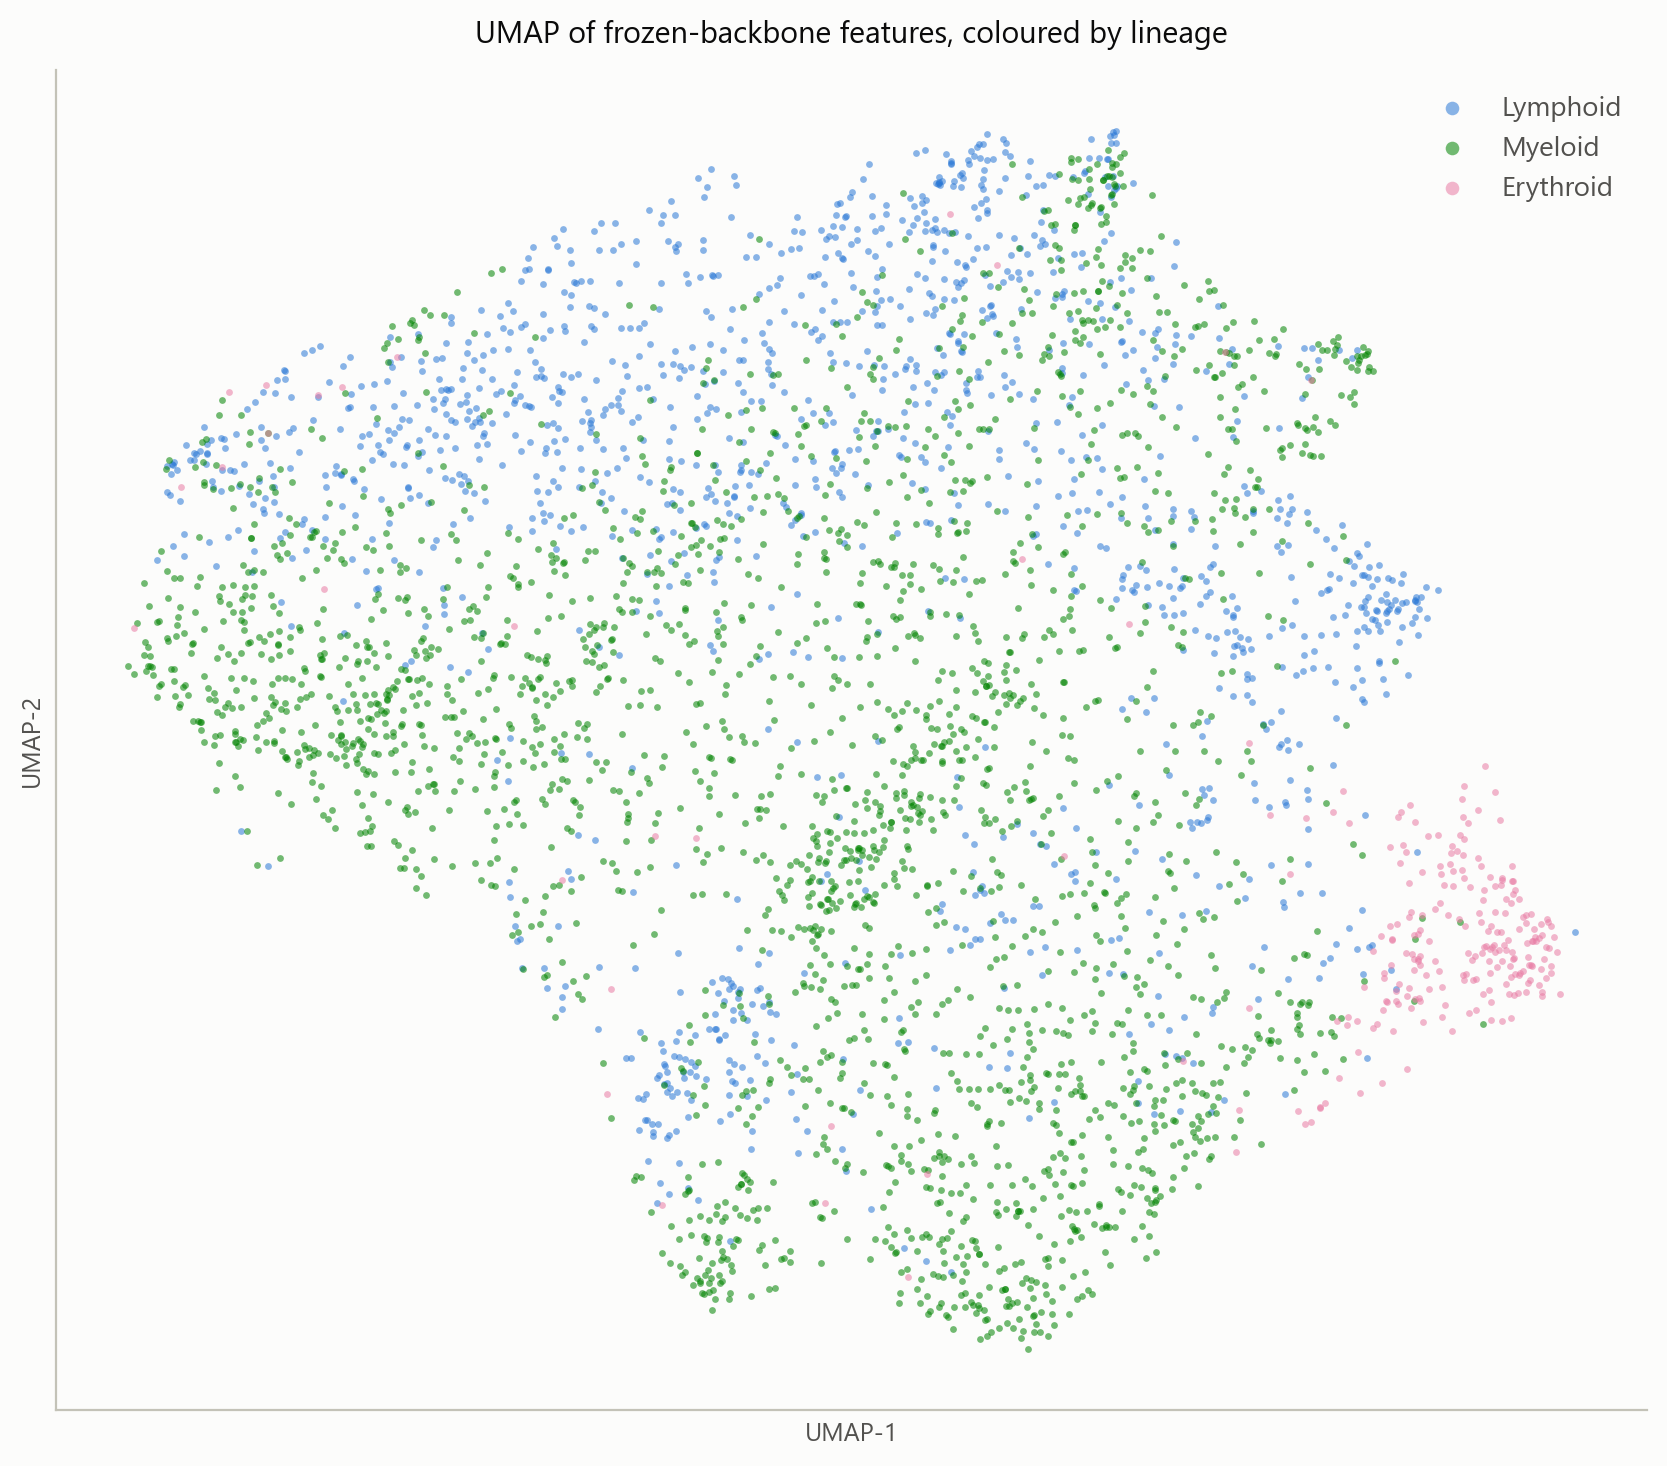
\includegraphics[width=0.84\linewidth]{umap_lineage.png}

      \vspace{0.2em}
      {\scriptsize Lineages overlap heavily in frozen ImageNet features. This
      justifies lineage as a \emph{soft regulariser}, and rules out a hard
      per-lineage routing gate.\par}
    \end{column}
  \end{columns}
\end{frame}

% ---------------------------------------------------------------- Slide 4
\begin{frame}{The first matrix (v1) --- and why we are running it again}
  \begin{columns}[T]
    \begin{column}{0.55\textwidth}
      \scriptsize
      \textbf{v1 results --- ViT, budget 50 epochs, early stopping on:}
      \smallskip

      \begin{tabular}{@{}lccc@{}}
        \toprule
        \textbf{Arm} & \textbf{Epochs survived} & \textbf{Macro F1} & \textbf{Minority F1} \\
        \midrule
        Hierarchical   & 37, 20, 29 & 0.853 & 0.791 \\
        Flat baseline  & 14, 13, 35 & 0.845 & \textbf{0.819} \\
        Stain-normalised & 21, 14, 12 & 0.824 & 0.758 \\
        No imbalance term & 13, 12, 12 & 0.824 & 0.711 \\
        \bottomrule
      \end{tabular}

      \medskip
      \textbf{The numbers looked publishable. They were not usable.}

      \smallskip
      \begin{itemize}\setlength{\itemsep}{0.25em}
        \item \textbf{Run length, not method, drove the score.}
          $\mathrm{corr}(\text{epochs run},\ \text{macro F1}) = \bad{+0.87}$.
          The arm ranking is nearly the ranking of epoch counts.
        \item \textbf{The learning-rate schedule was truncated.} Cosine was
          defined over 50 epochs but stopping fired at 12--37, leaving runs at
          up to \textbf{86\% of peak LR} --- never annealed. The 6-epoch screen
          runs scored \emph{higher} than any 50-epoch run.
        \item \textbf{Early stopping fired on noise.} Validation macro F1 moved
          sd $\mathbf{0.021}$ between epochs while the effects under study were
          $0.008$--$0.028$. \bad{The measurement noise exceeded the effect.}
      \end{itemize}
    \end{column}
    \begin{column}{0.43\textwidth}
      \centering
      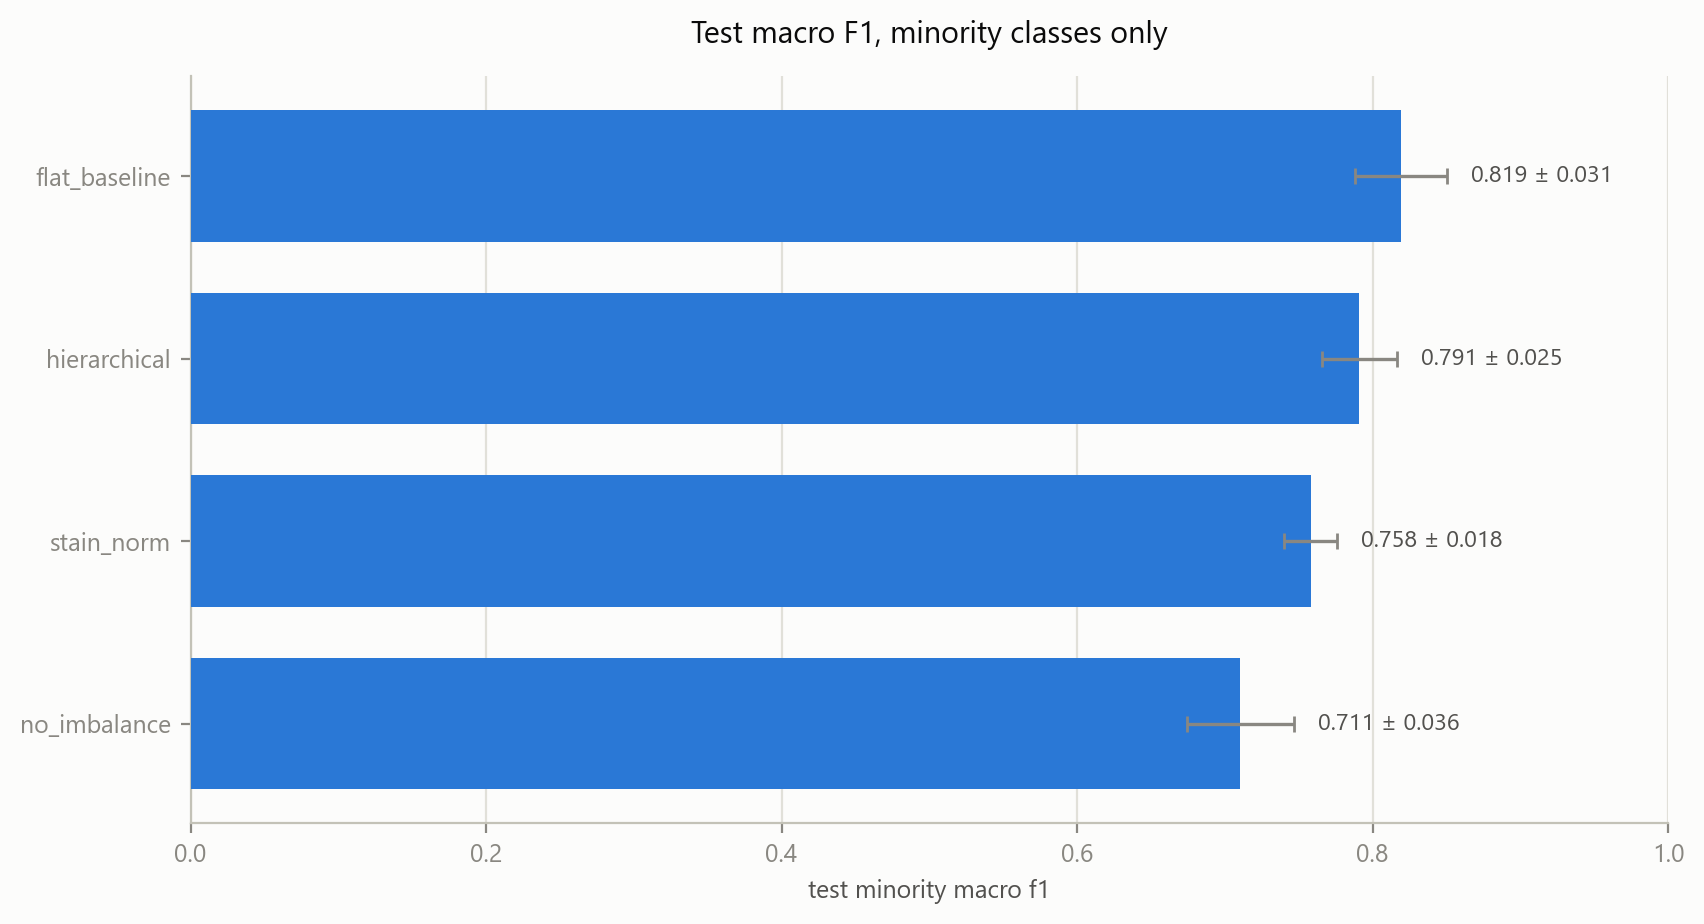
\includegraphics[width=0.94\linewidth]{arm_minority_f1.png}

      \vspace{0.2em}
      {\scriptsize \textbf{What v1 claimed.} The flat baseline ranked
      \emph{above} the hierarchical model on the rare classes --- the opposite
      of what v2 shows. That reversal is what the confound was worth.\par}

      \vspace{0.3em}
      \begin{alertblock}{Why re-run}
        \scriptsize
        No number of extra seeds could rescue v1: the noise was larger than the
        effect. The protocol had to change before any comparison could mean
        anything.
      \end{alertblock}
    \end{column}
  \end{columns}
\end{frame}

% ---------------------------------------------------------------- Slide 5
\begin{frame}{v1 $\rightarrow$ v2 --- what changed, and what it bought}
  \begin{columns}[T]
    \begin{column}{0.52\textwidth}
      \scriptsize
      \textbf{Protocol changes:}
      \smallskip

      \begin{tabular}{@{}p{3.1cm}p{4.0cm}@{}}
        \toprule
        \textbf{Change} & \textbf{Why} \\
        \midrule
        Early stopping \textbf{off}, fixed 30-epoch budget & Cosine always completes; every arm gets an identical anneal \\
        \addlinespace[0.2em]
        Weight \textbf{EMA} (0.999), evaluated instead of live weights & Halves the selection-metric noise \\
        \addlinespace[0.2em]
        \textbf{TTA} over four flip views & Cells have no canonical orientation \\
        \addlinespace[0.2em]
        \textbf{RandAugment + CutMix} on & Training loss had fallen to 0.005 against a 0.84 plateau --- plain memorisation \\
        \addlinespace[0.2em]
        \texttt{aug\_policy} threaded to the dataset & It was a dead config field; v1's column was fiction \\
        \bottomrule
      \end{tabular}
    \end{column}
    \begin{column}{0.46\textwidth}
      \scriptsize
      \textbf{Measured on one matched config} (hierarchical / ViT / seed 0 ---
      identical data, identical seed):
      \smallskip

      \begin{tabular}{@{}lccc@{}}
        \toprule
        \textbf{Metric} & \textbf{v1} & \textbf{v2} & $\Delta$ \\
        \midrule
        Test macro F1        & 0.8695 & 0.8809 & \good{$+0.011$} \\
        Balanced accuracy    & 0.8797 & 0.8929 & \good{$+0.013$} \\
        Minority macro F1    & 0.8201 & 0.8370 & \good{$+0.017$} \\
        Cross-lineage error  & 0.0133 & 0.0119 & \good{$-0.001$} \\
        Within-lineage error & 0.0413 & 0.0307 & \good{$-0.011$} \\
        \midrule
        \textbf{Val F1 epoch-to-epoch sd} & \textbf{0.0211} & \textbf{0.0097} & \good{$\mathbf{-54\%}$} \\
        \bottomrule
      \end{tabular}

      \medskip
      \begin{exampleblock}{The point}
        \scriptsize
        The accuracy gain is modest. \textbf{Halving the measurement noise is
        the real win} --- it is what makes an effect of $0.005$--$0.017$
        detectable at all. Cost: ${\sim}101$ s/epoch versus v1's ${\sim}60$ s.
      \end{exampleblock}
    \end{column}
  \end{columns}
\end{frame}

% ---------------------------------------------------------------- Slide 8
\begin{frame}{Results so far --- v2 matrix, ViT, 30 epochs}
  \centering
  \small
  \begin{tabular}{@{}lccccc@{}}
    \toprule
    \textbf{Arm} & \textbf{Seeds} & \textbf{Macro F1} & \textbf{Minority F1}
      & \textbf{Minority recall} & \textbf{Balanced acc.} \\
    \midrule
    Hierarchical (proposed) & 3 & \good{0.879 $\pm$ 0.003} & \good{0.840 $\pm$ 0.007} & \good{0.799} & \good{0.894} \\
    Flat baseline           & 3 & 0.874 $\pm$ 0.006 & 0.823 $\pm$ 0.014 & 0.776 & 0.883 \\
    No imbalance term       & 2 & 0.870 $\pm$ 0.010 & \bad{0.771 $\pm$ 0.031} & \bad{0.716} & \bad{0.859} \\
    Stain-normalised        & 0 & \multicolumn{4}{c}{\emph{currently training}} \\
    \bottomrule
  \end{tabular}

  \vspace{0.8em}
  \begin{columns}[T]
    \begin{column}{0.48\textwidth}
      \begin{exampleblock}{Hierarchical vs.\ flat (paired, by seed)}
        \small
        Macro F1 \quad $+0.005$, \; $p = 0.42$, \; $d_z = 0.57$ \\
        Minority F1 \; $+0.017$, \; $p = 0.29$, \; $d_z = 0.84$
      \end{exampleblock}
    \end{column}
    \begin{column}{0.48\textwidth}
      \begin{alertblock}{Reading}
        \small
        The proposed model wins on every metric, and by more on the rare
        classes than overall --- which is the predicted pattern. But with
        $n = 3$ seeds nothing reaches significance. The effect sizes are
        moderate-to-large; the \emph{sample of runs} is the limitation.
      \end{alertblock}
    \end{column}
  \end{columns}
\end{frame}

% ---------------------------------------------------------------- Slide 7
\begin{frame}{What the v2 numbers tell us}
  \small
  \begin{columns}[T]
    \begin{column}{0.48\textwidth}
      \begin{block}{1. The imbalance term is doing the real work}
        \scriptsize
        Removing it costs \bad{$-0.069$} minority macro F1 and \bad{$-0.083$}
        minority recall. That is an order of magnitude more than the hierarchy
        contributes ($+0.017$).

        \smallskip
        The imbalance-robust objective is the load-bearing component of the
        design --- which is a result worth reporting in its own right.
      \end{block}
    \end{column}
    \begin{column}{0.48\textwidth}
      \begin{alertblock}{2. The hierarchy is nearly inert by the end of training}
        \scriptsize
        Lineage accuracy saturates at \textbf{98.9\%}; both auxiliary losses
        collapse to ${\sim}0.0007$. The auxiliary task regularises an axis the
        model has \emph{already solved}, so it stops contributing gradient long
        before training ends.

        \smallskip
        This is a \emph{design} finding, not a tuning problem --- and it points
        directly at the fix on the last slide.
      \end{alertblock}
    \end{column}
  \end{columns}

  \vspace{0.6em}
  \begin{exampleblock}{Consistent with the exploratory analysis}
    \scriptsize
    Notebook 02 already found lineage separability to be local, not global, and
    the fine level far harder ($k$-NN agreement $0.78$ for lineage versus
    $0.42$ for cell type). The hard problem is discrimination \emph{within} a
    lineage --- myeloid maturation stages and the rare lymphoid types --- which
    is exactly where per-class F1 still collapses.
  \end{exampleblock}
\end{frame}

% ---------------------------------------------------------------- Slide 8
\begin{frame}{Problem 1 --- the imbalance is still the failure mode}
  \centering
  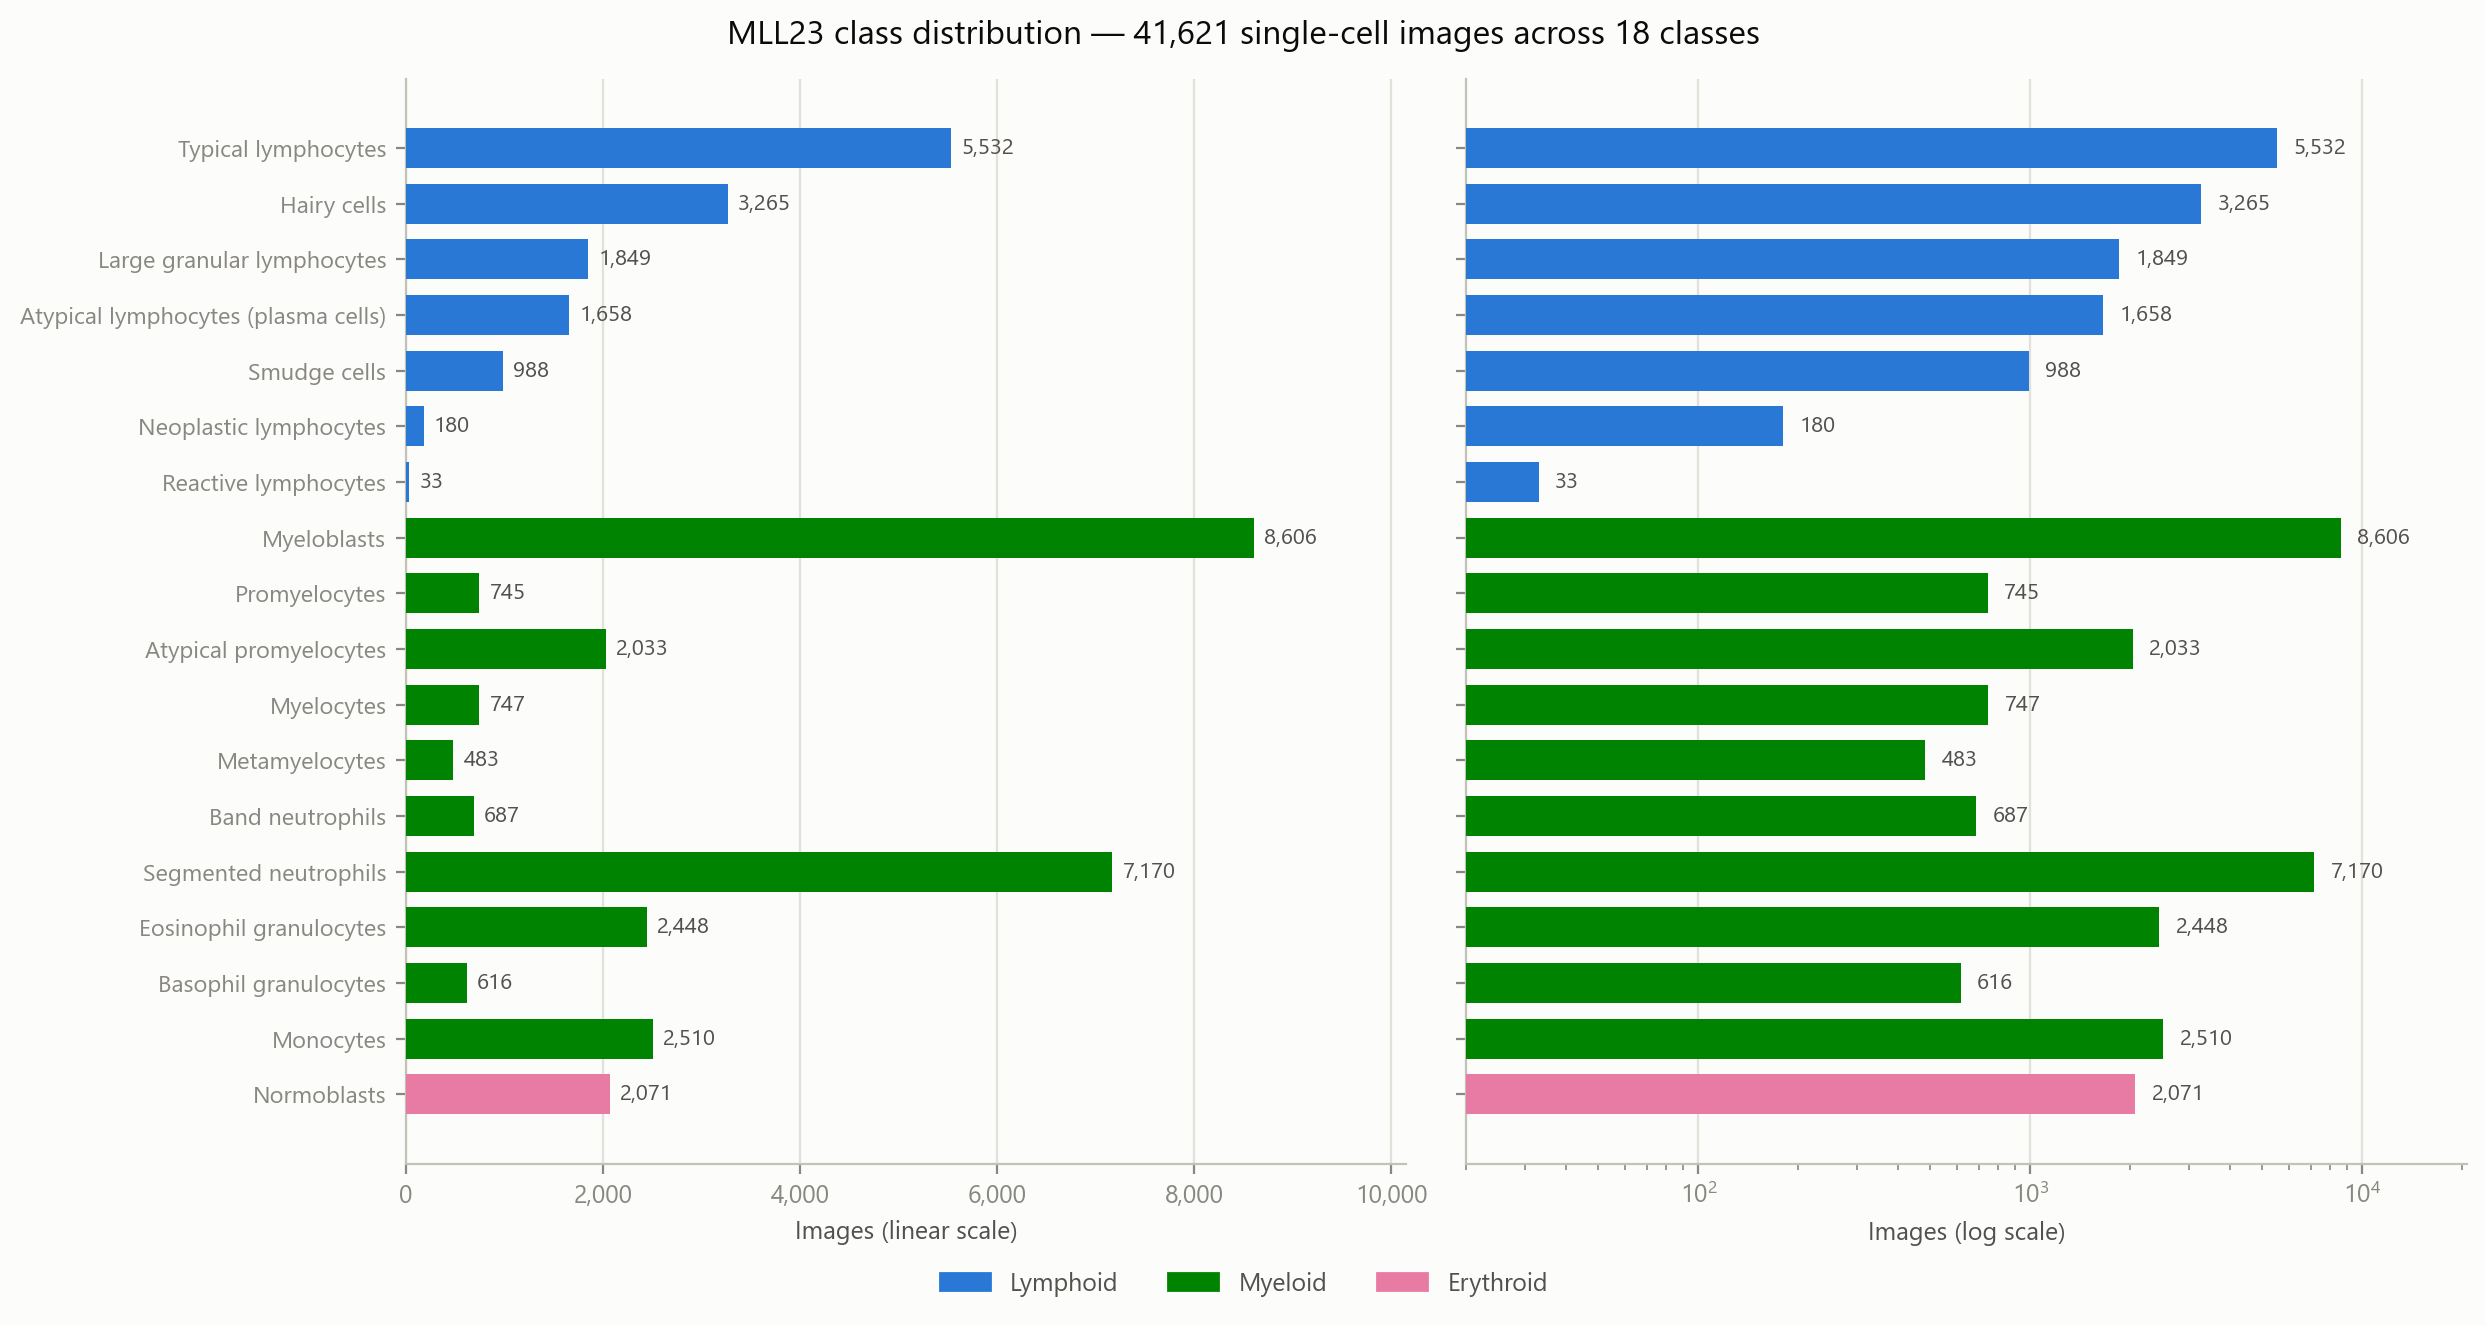
\includegraphics[width=0.60\linewidth]{class_distribution.png}

  \vspace{0.3em}
  \begin{columns}[T]
    \begin{column}{0.48\textwidth}
      \begin{alertblock}{The tail}
        \scriptsize
        \textbf{261:1} --- myeloblasts (8,606) to reactive lymphocytes (33),
        which leaves roughly \textbf{23 training images}. Minority recall is
        stuck at \textbf{0.80}.
      \end{alertblock}
    \end{column}
    \begin{column}{0.48\textwidth}
      \begin{block}{Where F1 collapses}
        \scriptsize
        Reactive lymphocytes ($\approx 0.55$); metamyelocytes, myelocytes, band
        neutrophils ($0.59$--$0.72$) --- the tail \emph{and} the adjacent
        maturation stages.
      \end{block}
    \end{column}
  \end{columns}
\end{frame}

% ---------------------------------------------------------------- Slide 7
\begin{frame}{Next --- scale up the experiments}
  \begin{columns}[T]
    \begin{column}{0.54\textwidth}
      \scriptsize
      \begin{tabular}{@{}lcc@{}}
        \toprule
        \textbf{Work} & \textbf{Runs} & \textbf{Est.\ GPU} \\
        \midrule
        Finish v2 matrix & 4 & ${\sim}5$ h \\
        \quad (\texttt{no\_imbalance} s2, \texttt{stain\_norm} $\times$3) & & \\
        Raise 3 $\rightarrow$ 5 seeds on all arms & 8 & ${\sim}10$ h \\
        Full backbone comparison at 30 epochs & 9 & ${\sim}12$ h \\
        \quad (ResNet / ConvNeXt / MobileNet $\times$3) & & \\
        \midrule
        \textbf{Total} & \textbf{21} & \textbf{${\sim}27$ h} \\
        \bottomrule
      \end{tabular}

      \smallskip
      Spent so far: \textbf{16.6 GPU-hours} for 8 runs on an RTX 4070 Laptop.

      \smallskip
      The 6-epoch screen \emph{selected} a backbone; it is not the backbone
      \emph{comparison} the proposal promised. Full-length runs are needed to
      report that honestly.
    \end{column}
    \begin{column}{0.43\textwidth}
      \begin{block}{Why this matters}
        \scriptsize
        Three seeds gives \textbf{2 degrees of freedom}. Five seeds, combined
        with the halved measurement noise from EMA, is what turns the paired
        tests from indicative into informative.
      \end{block}
      \begin{alertblock}{Decision needed}
        \scriptsize
        27 h is feasible locally but strictly serial. A rented cloud GPU would
        parallelise it into a weekend.
      \end{alertblock}
    \end{column}
  \end{columns}
\end{frame}

% ---------------------------------------------------------------- Slide 8
\begin{frame}{Next --- fix the imbalanced-data problem}
  \footnotesize
  Priority order, cheapest and highest-leverage first:

  \smallskip
  \begin{enumerate}\setlength{\itemsep}{0.25em}
    \item \textbf{Decoupled training (cRT).} Learn the representation with
      instance-balanced sampling, then retrain \emph{only the classifier} with
      class-balanced sampling. Among the strongest long-tail methods, and it
      reuses the backbones already trained --- minutes per run, not hours.
    \item \textbf{Logit adjustment / LDAM margin loss.} Enforce larger decision
      margins for rare classes. A stronger lever than reweighting alone, and a
      drop-in replacement inside the existing \texttt{losses.py}.
    \item \textbf{Retarget the auxiliary task.} Lineage is solved at 98.9\%, so
      it gives no gradient late in training. Point the auxiliary head at
      \textbf{maturation stage within the myeloid branch}, where the residual
      confusion actually lives.
    \item \textbf{Conditional inference.} Factor
      $p(y_2 \mid x) = p(y_1 \mid x)\, p(y_2 \mid y_1, x)$ so the coarse decision
      genuinely constrains the fine one, rather than two heads coexisting on a
      shared trunk and being nudged toward agreement.
  \end{enumerate}

  \vspace{0.3em}
  \begin{columns}[T]
    \begin{column}{0.49\textwidth}
      \begin{exampleblock}{Target}
        \scriptsize
        Minority macro F1 $0.840 \rightarrow 0.88+$, and minority recall off the
        $0.80$ plateau, with $p < 0.05$ at 5 seeds.
      \end{exampleblock}
    \end{column}
    \begin{column}{0.49\textwidth}
      \begin{block}{Sequence}
        \scriptsize
        Finish v2 matrix $\rightarrow$ add cRT and logit adjustment as new arms
        $\rightarrow$ re-run at 5 seeds $\rightarrow$ results chapter.
      \end{block}
    \end{column}
  \end{columns}
\end{frame}

\end{document}
